\documentclass{article}
\usepackage[utf8]{inputenc}
\usepackage{graphicx}
\usepackage{amsmath}
\usepackage{enumitem}
\usepackage{multicol}
\usepackage{subcaption}

\usepackage{geometry}
\geometry{
 a4paper,
 total={170mm,257mm},
 left=20mm,
 top=20mm,
 }

\title{CSC411 Project\#2 Bonus}
\author{Yifei Dong \& Zifei Han}
\date{February 28th 2018}

\begin{document}

\maketitle

\section*{Figures}

\begin{figure*}[!ht]
\begin{subfigure}{.35\textwidth}
  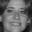
\includegraphics[width=.5\linewidth]{bracco2.jpg}
  \caption{Bracco}
  \label{fig:sfig1}
\end{subfigure}
\begin{subfigure}{.35\textwidth}
  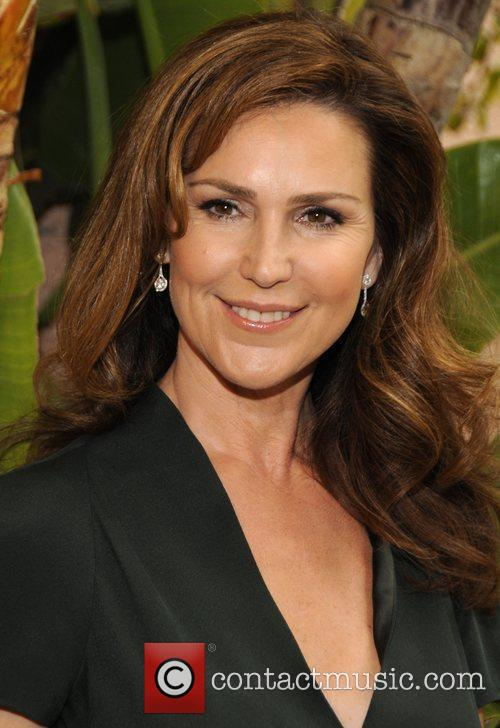
\includegraphics[width=.5\linewidth]{gilpin2.jpg}
  \caption{Gilpin}
  \label{fig:sfig2}
\end{subfigure}%
\begin{subfigure}{.35\textwidth}
  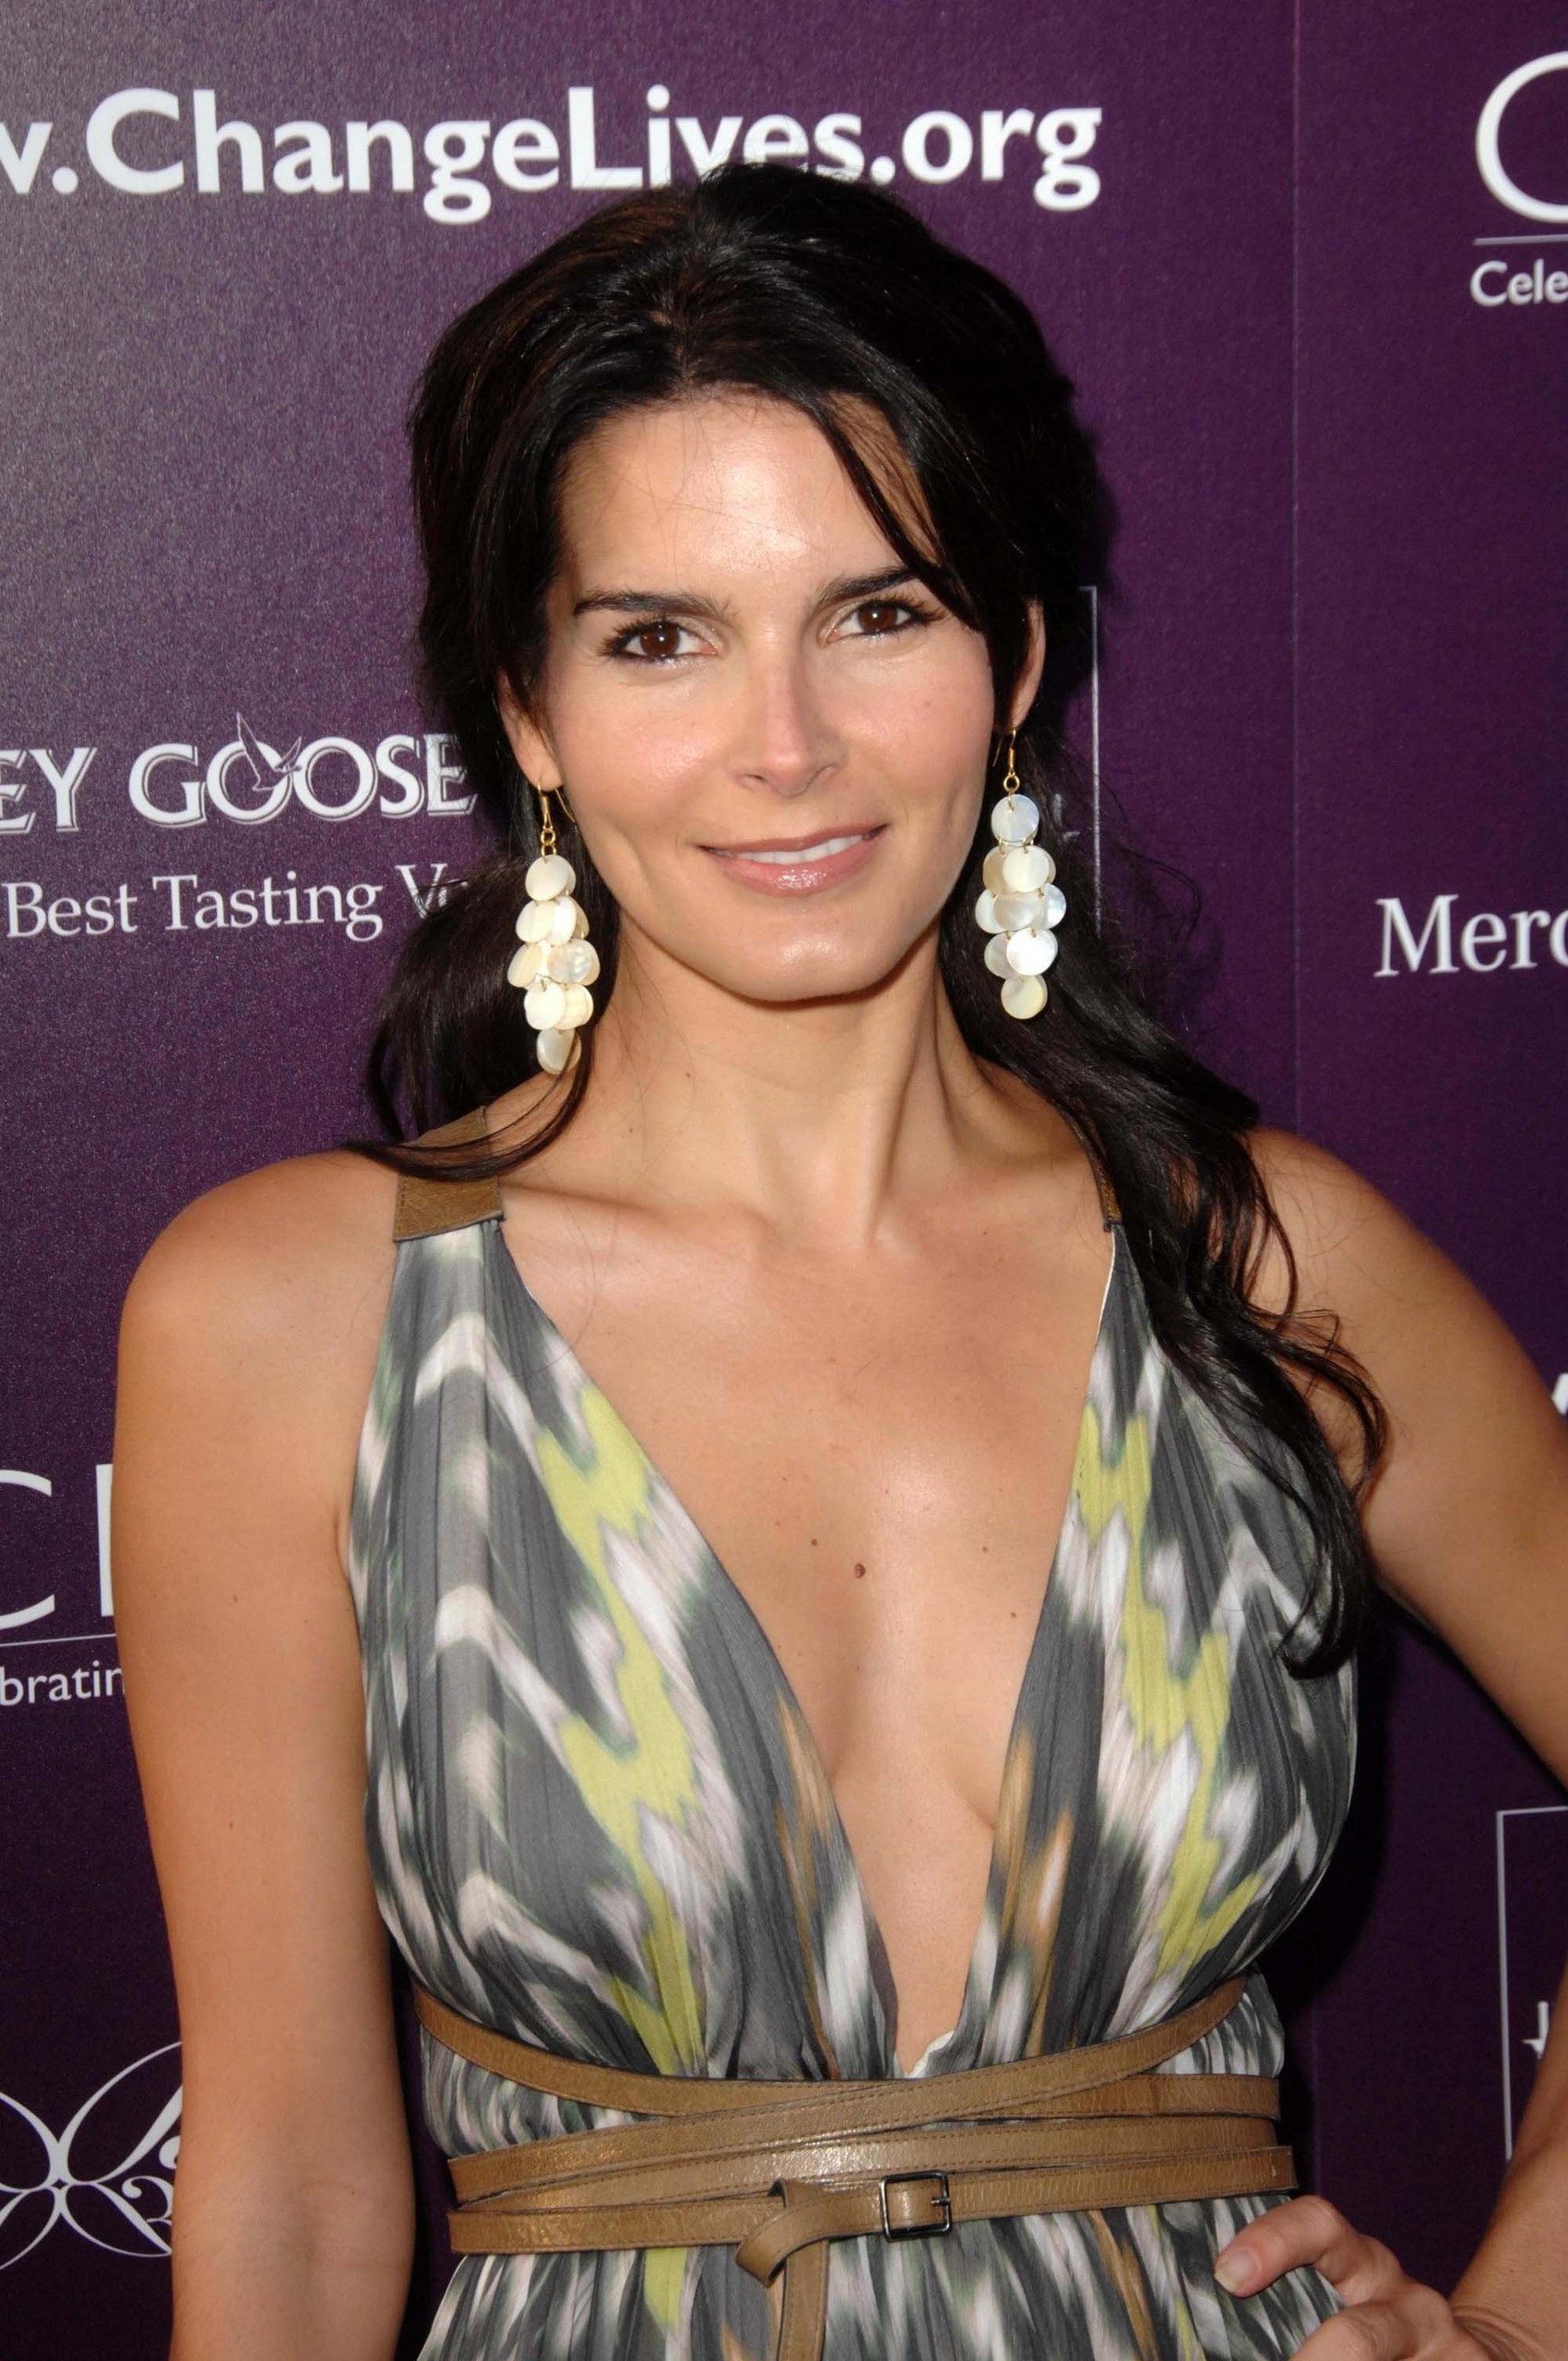
\includegraphics[width=.5\linewidth]{harmon3.jpg}
  \caption{Harmon}
  \label{fig:sfig3}
\end{subfigure}
\begin{subfigure}{.35\textwidth}
  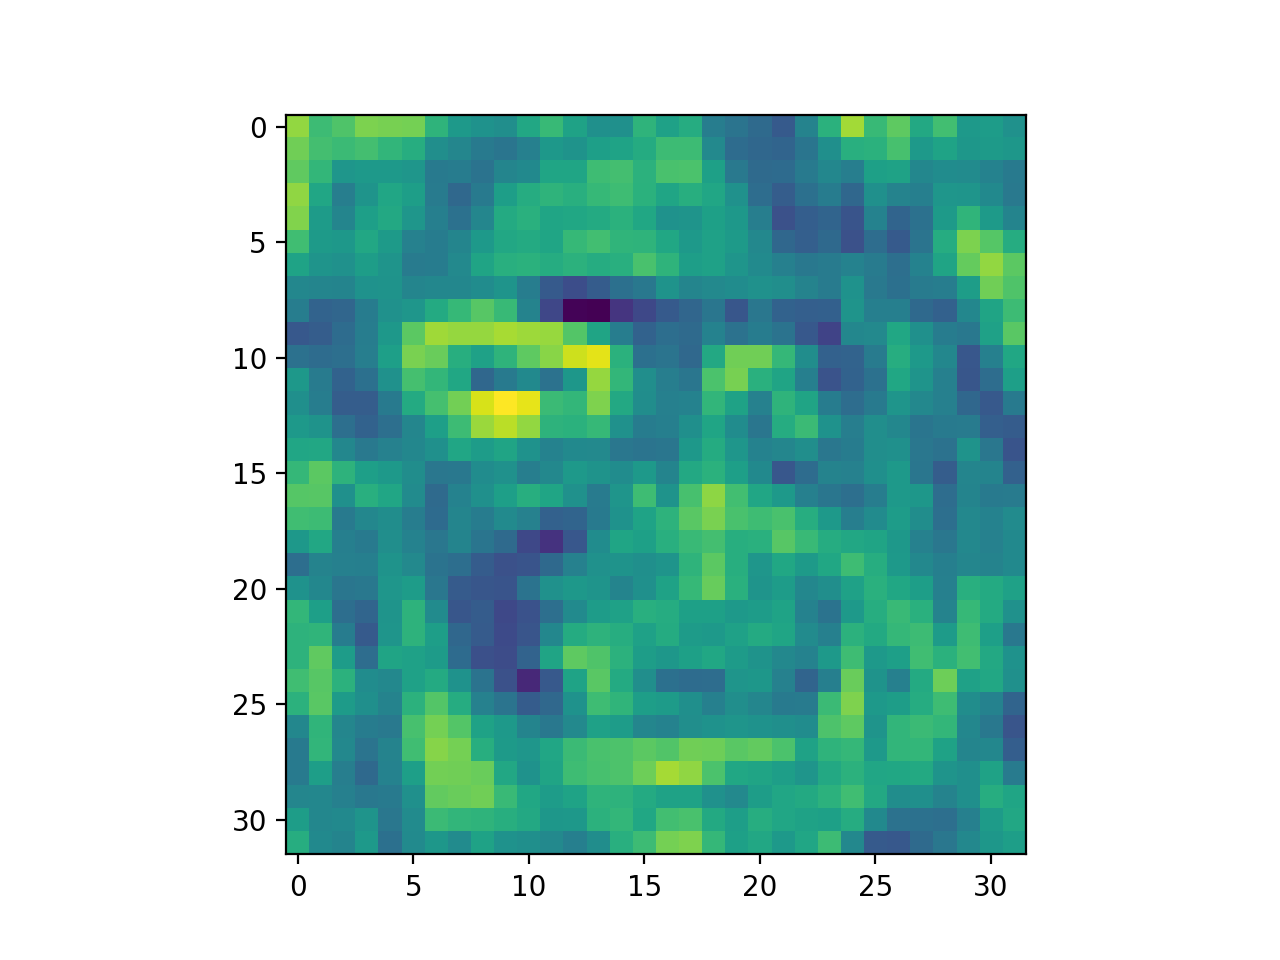
\includegraphics[width=.8\linewidth]{bracco.png}
  \caption{Bracco}
  \label{fig:sfig4}
\end{subfigure}%
\begin{subfigure}{.35\textwidth}
  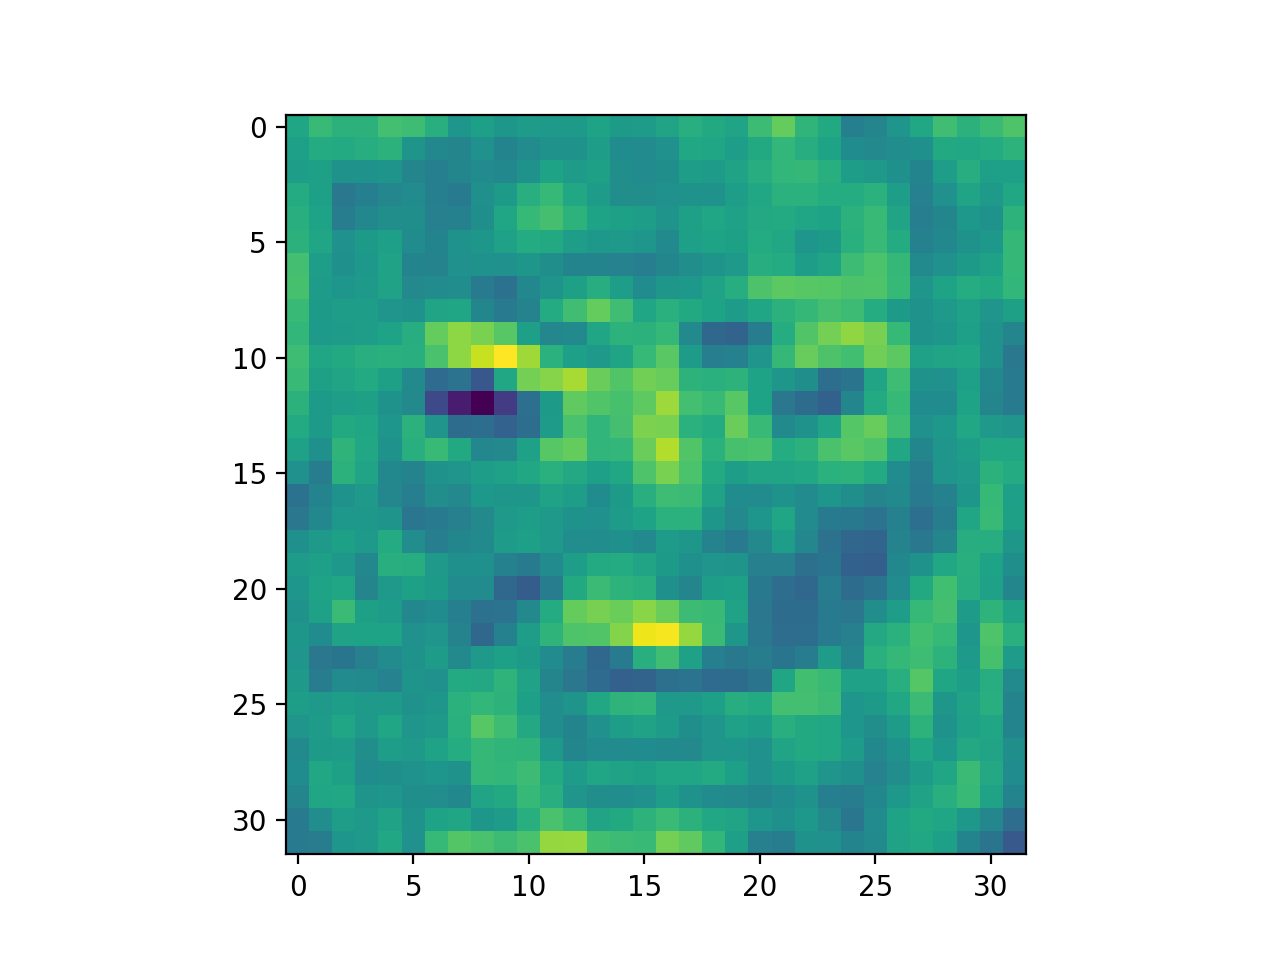
\includegraphics[width=.8\linewidth]{gilpin.png}
  \caption{Gilpin}
  \label{fig:sfig5}
\end{subfigure}
\begin{subfigure}{.35\textwidth}
  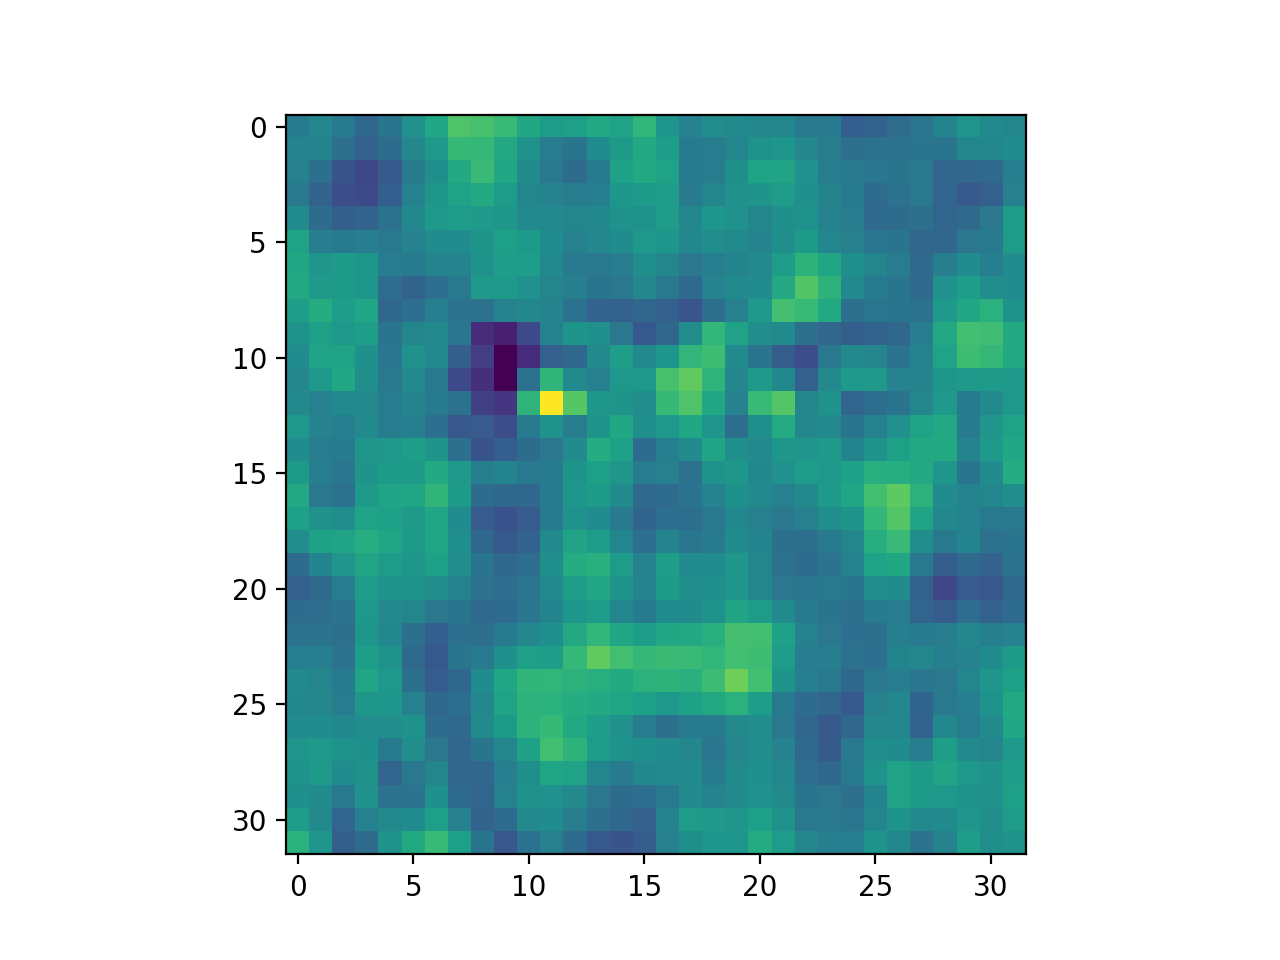
\includegraphics[width=.8\linewidth]{harmon.png}
  \caption{Harmon}
  \label{fig:sfig6}%
\end{subfigure}
\caption{}
\label{fig:pcs}
\end{figure*}

\begin{figure*}[!ht]
\begin{subfigure}{.35\textwidth}
  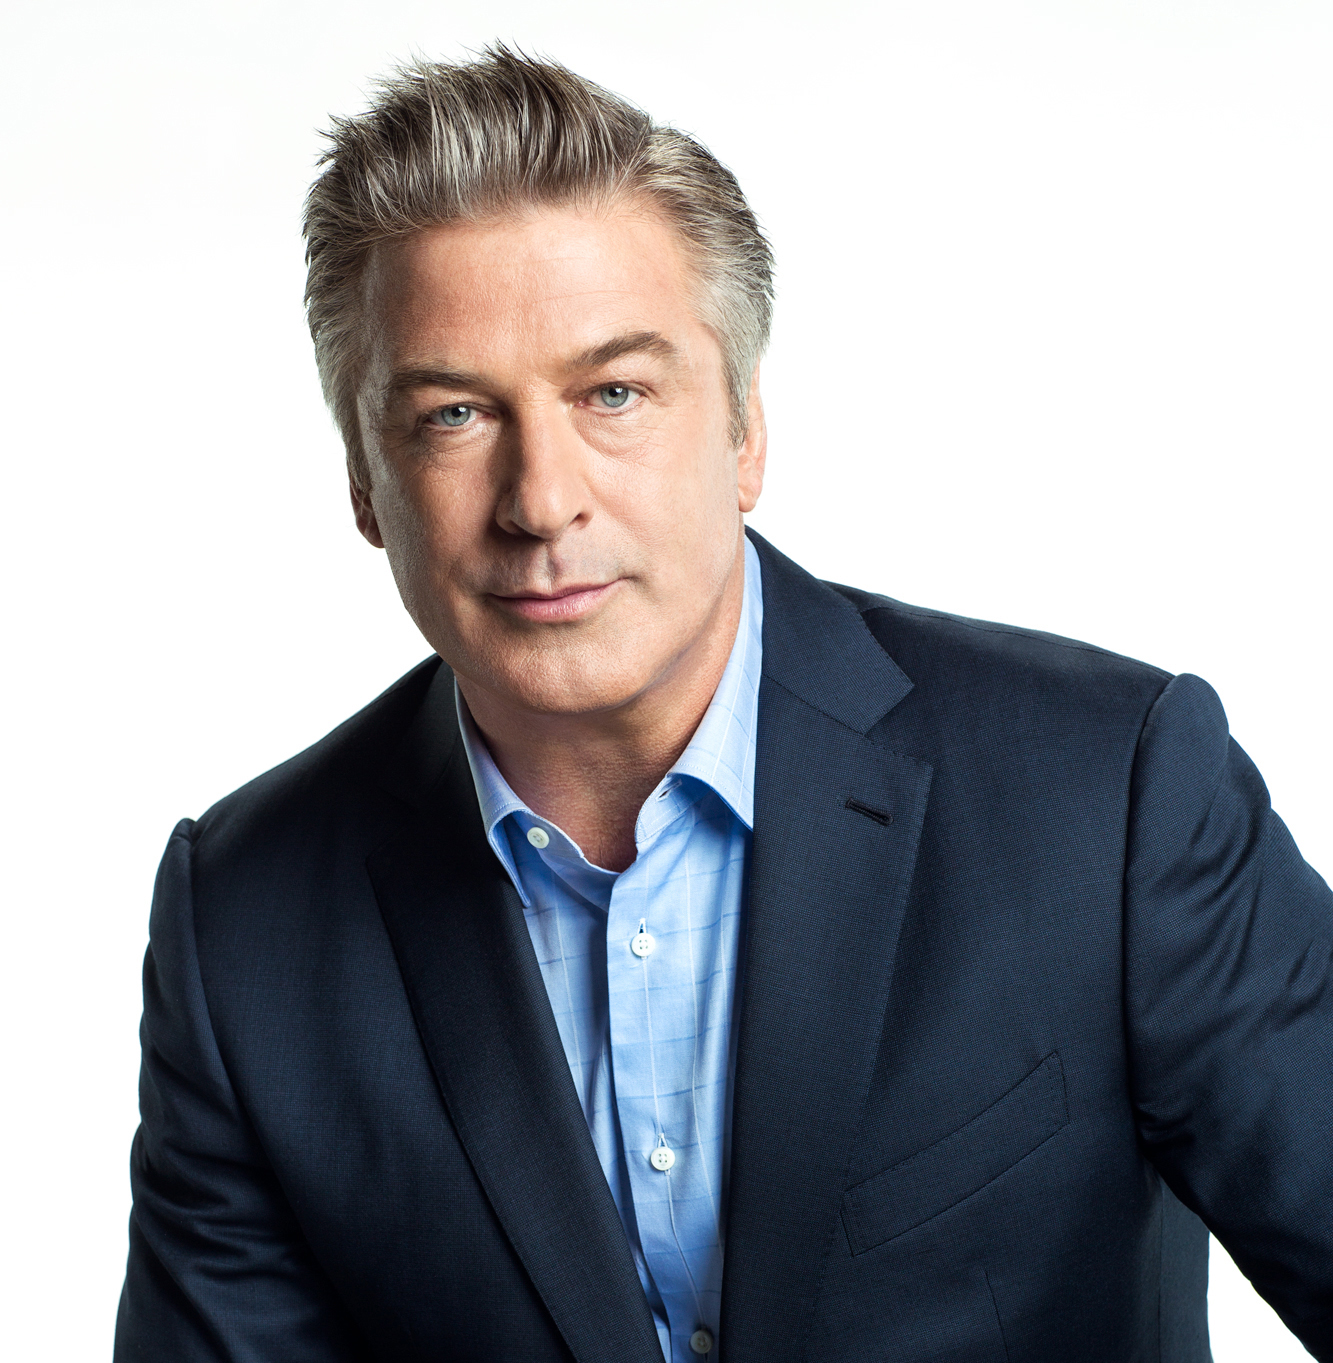
\includegraphics[width=.5\linewidth]{baldwin3.jpg}
  \caption{Baldwin}
  \label{fig:sfig7}
\end{subfigure}
\begin{subfigure}{.35\textwidth}
  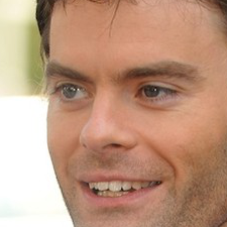
\includegraphics[width=.5\linewidth]{hader3.jpg}
  \caption{Hader}
  \label{fig:sfig8}
\end{subfigure}%
\begin{subfigure}{.35\textwidth}
  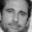
\includegraphics[width=.5\linewidth]{carell4.jpg}
  \caption{Carell}
  \label{fig:sfig9}
\end{subfigure}
\begin{subfigure}{.35\textwidth}
  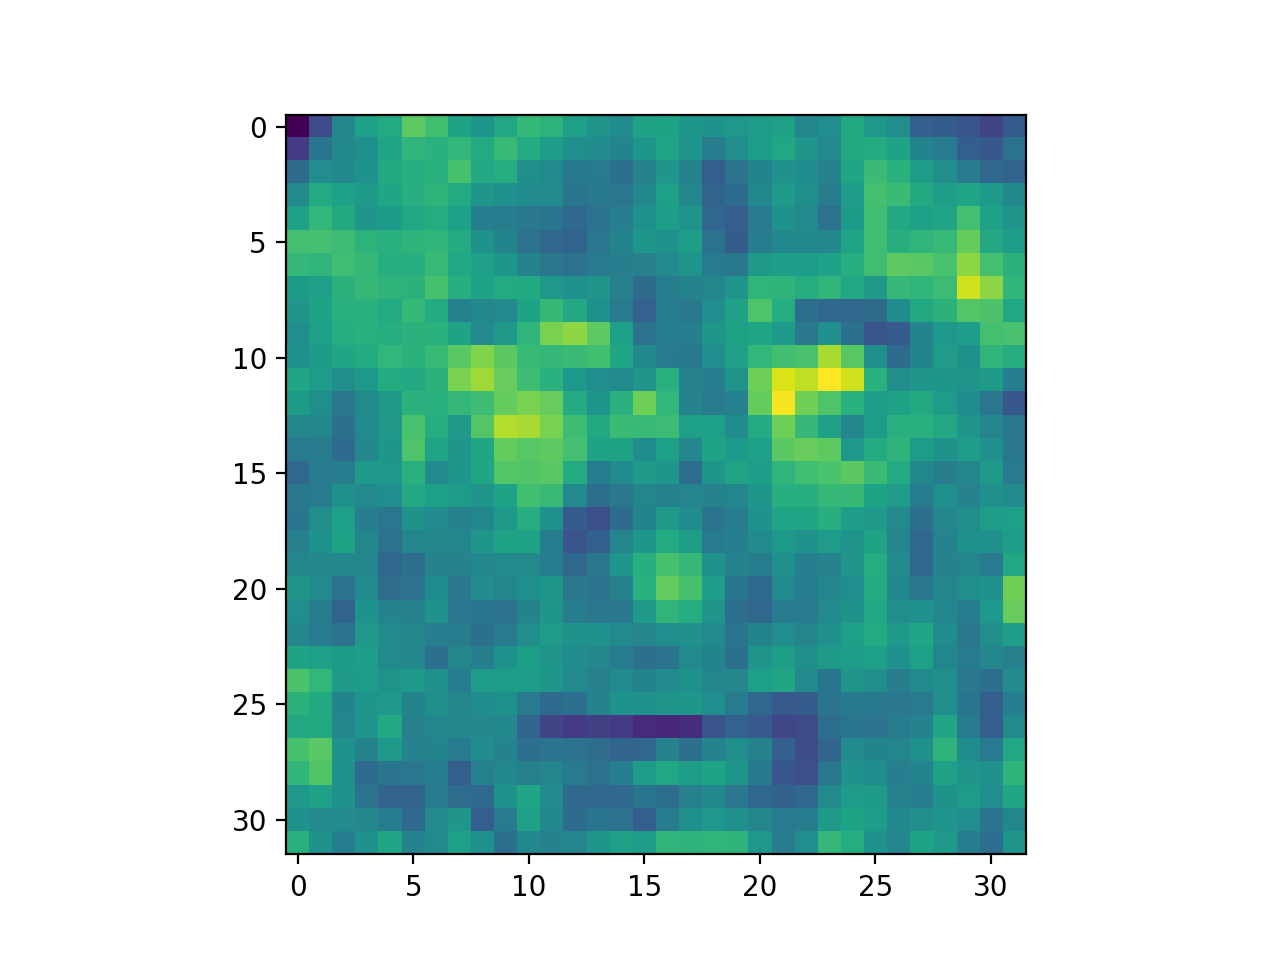
\includegraphics[width=.8\linewidth]{baldwin.png}
  \caption{Baldwin}
  \label{fig:sfig10}
\end{subfigure}%
\begin{subfigure}{.35\textwidth}
  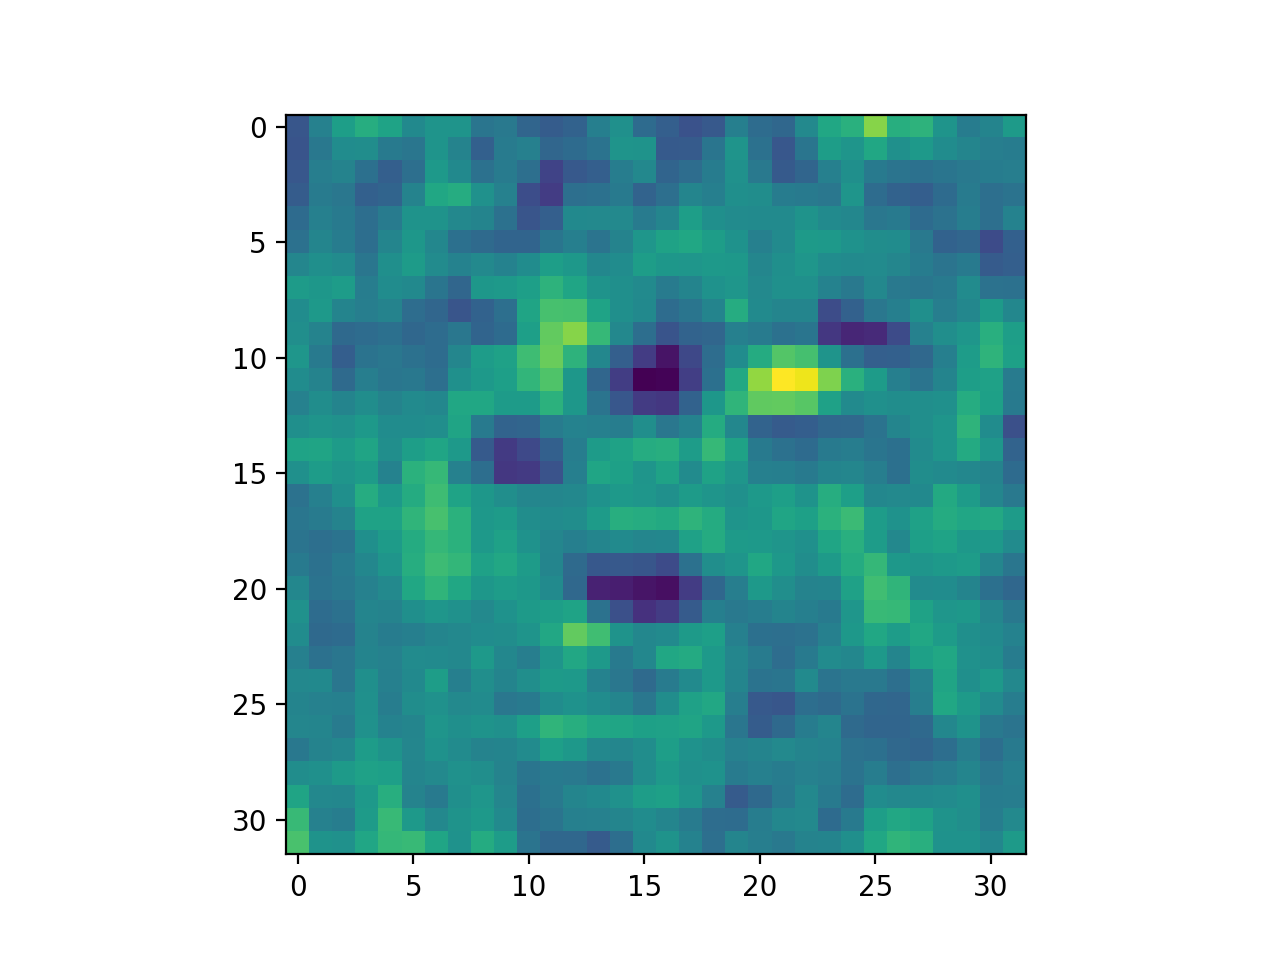
\includegraphics[width=.8\linewidth]{hader.png}
  \caption{Hader}
  \label{fig:sfig11}
\end{subfigure}
\begin{subfigure}{.35\textwidth}
  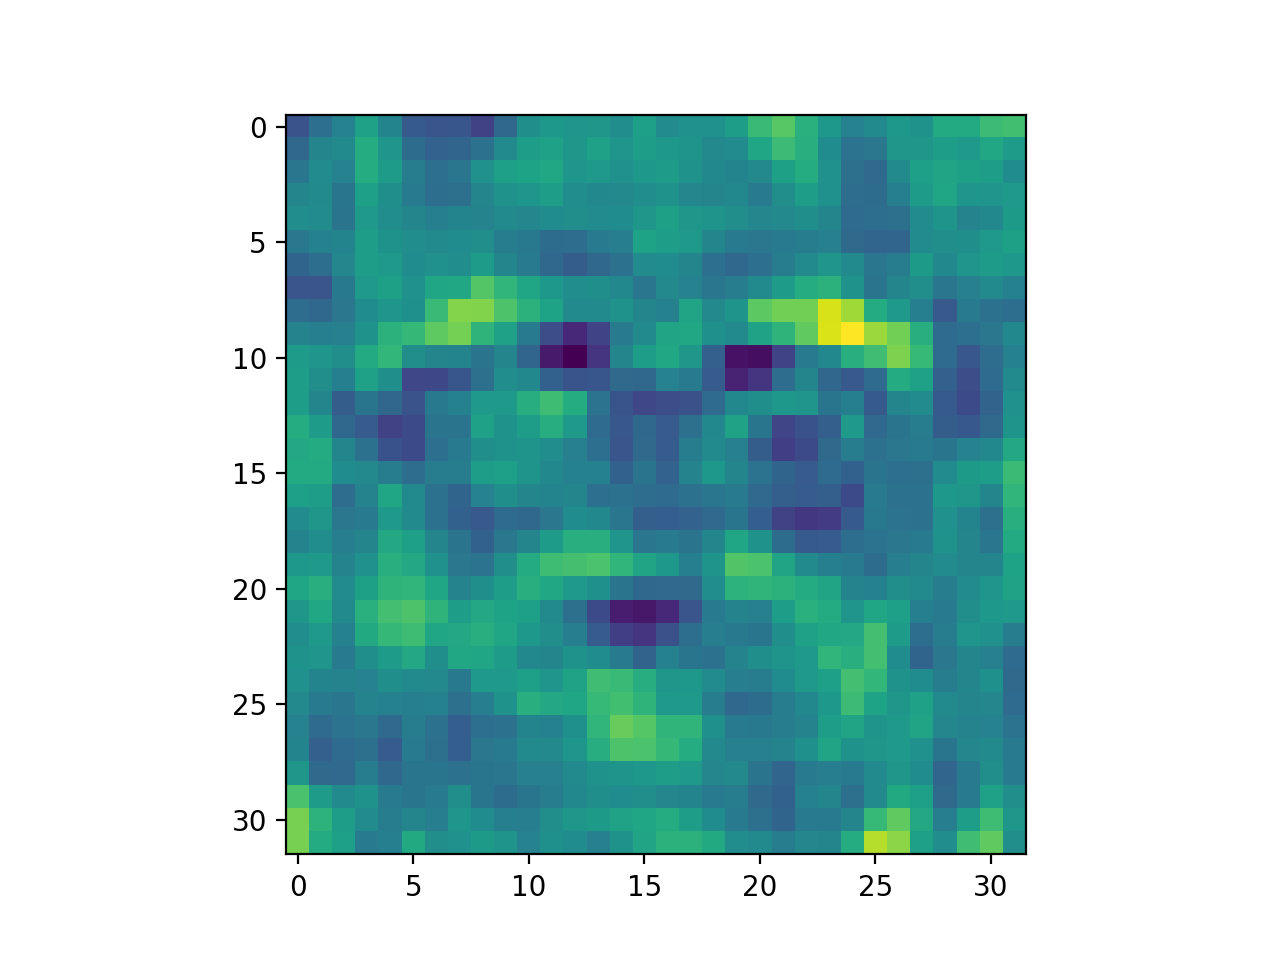
\includegraphics[width=.8\linewidth]{carell.png}
  \caption{Carell}
  \label{fig:sfig12}%
\end{subfigure}
\caption{}
\label{fig:pcs1}
\end{figure*}
\clearpage
\begin{figure*}[!ht]
\begin{subfigure}{.35\textwidth}
  
\includegraphics[width=.5\linewidth]{uoft.jpeg}
  \caption{U of T}
  \label{fig:uoft}
\end{subfigure}
\begin{subfigure}{.35\textwidth}
  
\includegraphics[width=.5\linewidth]{face1.jpeg}
  \caption{face1}
  \label{fig:face1}
\end{subfigure}%
\begin{subfigure}{.35\textwidth}
  
\includegraphics[width=.5\linewidth]{face2.jpeg}
  \caption{face2}
  \label{fig:face2}
\end{subfigure}
\begin{subfigure}{.35\textwidth}
  
\includegraphics[width=.8\linewidth]{uoft.png}
  \caption{U of T}
  \label{fig:uoft1}
\end{subfigure}%
\begin{subfigure}{.35\textwidth}
  
\includegraphics[width=.8\linewidth]{face1.png}
  \caption{face1}
  \label{fig:face11}
\end{subfigure}
\begin{subfigure}{.35\textwidth}
  
\includegraphics[width=.8\linewidth]{face2.png}
  \caption{face2}
  \label{fig:face21}%
\end{subfigure}
\caption{}
\label{fig:pcs2}
\end{figure*}

\subsection*{Conclusion}
We have drawn the pictures for the last layer in AlexNet features, which is MaxPool2d. We can see that all the faces have similar plots during the layer. The lightening pixel locations are very similar.\\
To compare, we tried to train the algorithm with u of t logo and some fake smiley faces. We can see a huge change in U of T logo's Max Pool layer's plot, while the smiley faces have somewhat similar. 



\end{document}
